\documentclass{article}
\usepackage{graphicx}
\usepackage[margin=1in]{geometry}
\parskip=2mm
\title{Coursework 1: Methods and Plans}
\author{Group 31}
\begin{document}
\maketitle
The project which we were assigned was initially entitled “Eye Capture Window Manager”.  The aim of which is to create a piece of window management software that integrates with a linux operating system.  This should use eye tracking to monitor the user’s gaze and in turn which window is being looked at and switch focus accordingly.
\section*{Method}
We decided to choose Kanban after having examined other agile methods that were available to us.  We chose Kanban as it is more flexible than the methodologies of XP or Scrum, they are both more prescriptive in either teams and meetings or having practices that must be kept to every iteration.  The Kanban board is an incredibly useful tool in tracking the development time of features and learning how this can be made more efficient: finding the bottlenecks in the process.  Having this visualisation means that all members of the team know where each feature is in the development process.  No member of the team has a particularly large specialisation in a certain area, so this means everybody can be involved, to a certain extent, on the implementation of each feature when need be. It is also markedly different to the methodologies that most members of the group have used in previous group projects, and therefore provides a good opportunity to try something new to increase productivity.

The potential scope of the project is very large, but our team has a strictly limited set of resources to complete it.  This is another reason we chose Kanban, as it’s limit of the amount of work in progress at a particular time means the team will not be overwhelmed with features in the development process.   Without a similar methodology, our fear was we could end up with many partly implemented features and an unfinished product. With it, we should be able to focus on the things we need to get working first, then move onto the smaller and perimeter features,

Another important aspect of our project is that none of us, or even our Supervisor, have a particular idea of how difficult or time consuming each step will be. Kaban encourages constant small changes over time in comparison to larger changes in one sprint or cycle.  This means the project, which is still young and we are yet to fully understand, will be agile to changing requirements which we will most definitely encounter as we begin to implement.

\clearpage
We are using the website ‘Trello’ as a Kanban board to track the progression of features through the development cycle.  While this website is not specifically designed for this purpose, it provides the facilities to do so: columns in which tasks can be pinned and dragged from one to the other.  The categories we are currently using are named as follows:

\begin{itemize}
\item TODO: features that are yet to be started
\item Analysis: analysing how the feature should be implemented
\item Doing: features currently in development
\item QA: features going through testing
\item Done: features that are complete, left on the board in case future issues occur that move them back down
\end{itemize}

The screenshot included shows our current project on the website with a couple of cards added. \\[1mm]

{\centering
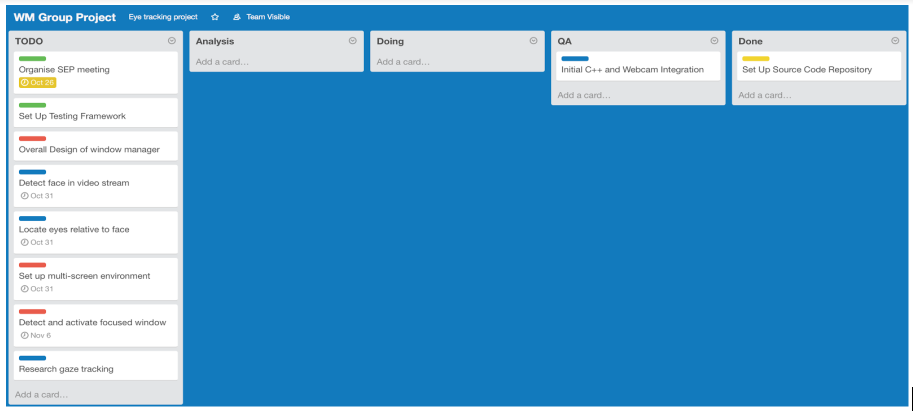
\includegraphics[scale=0.35]{trello.png}\par
}

\vspace*{2mm}
The team still has regular meetings in addition to subscribing to the Kanban methodology.  This allows face-to-face time with the group which is useful for having more complex discussions related to development or other issues.  A diary is kept of tasks achieved and problems encountered during these meetings so we have a history of how the project has progressed and how we have managed to deal with issues that we have encountered.

\section*{Plan}
We have split the group into 2 even sized sub teams (3 members each), one working on the eye tracking and the other working on switching windows/window management and user interface. This split makes sense in our context for two main reasons. First, the project is easily divisible (the two sides ought to be isolated anyway to maximise the potential of them both) and both sides will require large amounts of work from the start. Also, 3 members of the group are taking the Computer Vision course which will both support and be supported by the project, while the other members have chosen other options this term, which could potentially lead to problems in the more intensive areas of the eye tracking side of the project. Having said this, we anticipate the eye tracking to take longer, so the assignment of the subteams is flexible. 

This division lead us to the conclusion we should create to fairly separate programs, sharing very little, if any, internal details. The window team will have to provide an interface to change the focus of windows, and will design the communication between the apps. The eye tracking app will detect the user gaze, and convert its conclusions into messages to the window app. Splitting the implementation in this way allows the potential to use the components separately, for instance using the eye tracking system with other operating systems or other display servers, or building a system that detects another physical input which can change the focus of windows and be managed in the same way. 

\subsection*{Eye Tracking}
The plan is to start by tracking the user's face in order to detect which screen they are looking at. From meetings with our supervisor, we were directed to Aldo Faisal who has done previous work in areas similar to this. Due to his experience, he advised us that we should start with simple face detection rather than the precision of detecting the user’s gaze.  The “Viola-Jones” technique is one that was specifically motivated by the problem of face detection.

We expect to be able to use just a webcam for the face tracking and hope to continue without any extra equipment to track the user’s eyes. However our research has shown that using an infrared light source to illuminate the user’s eyes would allow the easier detection of the eyes due to the bright pupil effect. So we will evaluate the cost and availability compared to the benefit provided, aiming to use low cost, off the shelf equipment. As we move into the development and encounter these problems, we will be much better placed to work out whether we need to employ less standard hardware.

Development on this side has started by researching a library to use for the video processing. We discovered and decided to use the C++ library OpenCV, as it handles integration with multiple webcams, an interface to substitute video or photos in place of a webcam, defines easy to use templates for handling images, and even implements some of the image processing techniques we may need to use. We have successfully managed integration with a webcam, live frame by frame processing of the video stream it provides, and use of the GUI library that pairs with OpenCV (called highgui) to display the feed. We now plan to start working on face detection, and then inferring which direction a user is looking. Hopefully, this should be complete by week 6, but as none of us have done anything similar in the past, estimating these things is quite hard.

Once face detection by “Viola-Jones” is complete, we plan to look into more precise detection of where the user is looking. This will take three things: The detection of the eye, the tracking of the eye, and inferring where the eye is pointing. The first part, eye detection, can be tried on still images and needs a lot of experimentation and research to complete, as there are many methods people have successfully employed in the past. The second part of eye tracking management takes the form of tracking a detected eye frame to frame. As the position of the eye is known in the previous frame, this should make it easier to track to the next frame. The final part relies on the completion of the first two, and suggests the use of a lot more techniques to get the detection of exact gaze position from the images. We plan to have at least some precision of gaze position inference by the end of term, and will hopefully try to continue improving it over the christmas holidays. Cursory research has shown existing methods that track the pupil relative to another point such as a corneal reflection.

\subsection*{Window Management}
The window team works parallel with eye tracking team, but should finish earlier than eye tracking team. The team requires multi-screen computer, eye tracking data and Xlib module to do the task. Multi-screen computer is used for testing purpose, so code could be checked actively in early stage. Eye tracking data indicates the position and movement of the eye and it is used to analysis which screen is looked at. Xlib module is the main source in the task.

The timescale for the task is set and team members try to finish each part on time. On week 2 and week 3, we do background research and set up multi-screen computer. From week 4 to week 7, we analyse coordinates in 2D format, so that we can calculate the user focused window. This is the most challenging part and require intense knowledge about Xlib module. On week 8, we aim to send data to window manager and ask window manager change focus to the given window. At that time, the active window is mainly finished and should be tested intensively.

The task will need to take the information which has been gathered on the direction of the user’s gaze and change the window/screen which is in focus accordingly. Our initial development of the software will be implemented parallel with eye tracking and windows. Window team assumes there is real time eye tracking data and uses made-up data for testing purpose. It connects to eye tracking part once eye tracking is implemented.

The time is estimated based on previous work experience. The team members work on window management have cooperated many times and are familiar with working pace with each other. In addition, task is splitted to several small parts, so that it is easier to estimate the time for small part. Due to research at the beginning, we understand what to do in the project, so time is estimated sensibly.

On current stage, we have made design decision according to online resources. Initially, we plan to build a basic window manager and add eye building function to it. When we found there are actually many existing functional window manager, it appears overkill to implement all functions. Meanwhile, if we develop active window function based on one window manager, our final product is too limited for users. As a result, we decide to achieve active window by sending data to X server, so that it doesn’t interference with window manager. User can use our software together with their window manager. Also, we have built multi-screen computer in lab, which allows us to test the system.

\subsection*{User Interface}
Once the two technique parts: eye tracking and window management are all done and tested, we aim to create a user friendly interface:

Here’s a demo for user interface: \\[1mm]

{\centering
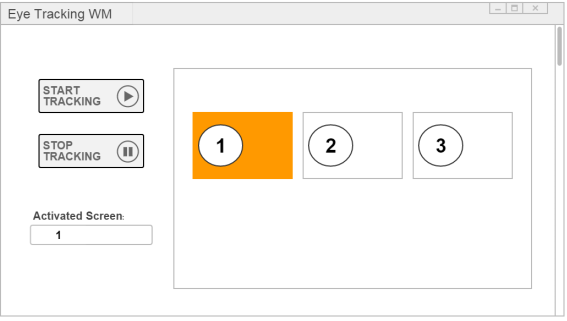
\includegraphics[scale=0.7]{ui.png}\par
}

\end{document}
